%LTeX: language=pt-br
% !TeX root = Apostila_IM381.tex

\cleardoublepage
\section{Elemento de viga}

    \subsection{Obtenção da forma fraca}

        Conforme visto na seção anterior, a equação diferencial do modelo de viga é:

        \begin{equation}
            EI_{zz}\frac{d^4v}{dx^4} = q(x).
        \end{equation}

        O procedimento a ser utilizado aqui para a aproximação é similar. Sabendo que a solução dessa equação se encontra com $v \in V$, propõe-se a utilização de uma função peso $w \in W$:

        \begin{equation}
            \int_0^L w EI_{zz}\frac{d^4v}{dx^4} dx - \int_0^L w q(x) dx = 0
        \end{equation}

       Da mesma forma como na barra, podemos aplicar integração por partes para chegar à forma fraca do problema de viga. Neste caso, entretanto, como estamos numa equação diferencial de ordem $4$, aplicaremos a integração por parte duas vezes:

        \begin{equation*}
            \int_0^L w EI_{zz}\frac{d^4v}{dx^4} dx = -\int_0^L \frac{dw}{dx} EI_{zz}\frac{d^3v}{dx^3} dx + \left[w EI_{zz}\frac{d^3v}{dx^3}\right]_0^L = -\int_0^L \frac{dw}{dx} EI_{zz}\frac{d^3v}{dx^3} dx + \left[w V_y\right]_0^L
        \end{equation*}

        \begin{equation}
            = \int_0^L \frac{d^2w}{dx^2} EI_{zz}\frac{d^2v}{dx^2} dx + \left[w V_y\right]_0^L - \left[\frac{dw}{dx} EI_{zz}\frac{d^2v}{dx^2}\right]_0^L = \int_0^L \frac{d^2w}{dx^2} EI_{zz}\frac{d^2v}{dx^2} dx + \left[w V_y\right]_0^L - \left[\frac{dw}{dx} M_z\right]_0^L
        \end{equation}

        Portanto, a equação final fica:

        \begin{equation}
            \int_0^L \frac{d^2w}{dx^2} EI_{zz}\frac{d^2v}{dx^2} dx = 
            -w(L) V_y(L) + w(0) V_y(0) + \theta_w(L)M_z(L) - \theta_w(0)M_z(0)+ \int_0^L w q(x) dx
        \end{equation}

        \noindent no qual $\theta_w = \frac{dw}{dx}$.


    \subsection{Polinômios de Hermite}

        No caso da viga, temos duas variáveis que devemos obter em cada ponto do domínio, sendo elas o deslocamento $v(x)$ e a rotação $\theta(x)$. Estas variáveis, no entanto, não são independentes entre si. Conforme mostrado na seção anterior, considerando pequenos deslocamentos e deformações, temos a relação entre elas:

        \begin{equation}
            \theta(x) = \frac{dv}{dx}
        \end{equation}

        Considere um elemento de viga da Figura \ref{fig:malha_viga}. No caso da viga, definem-se normalmente as coordenadas locais $\bar{x}$ como indo de 0 ao comprimento do elemento $h_e$ (Note que $\frac{dx}{d\bar{x}} = 1$). Em cada nó do elemento, há dois graus de liberdade, correspondentes às duas variáveis. O deslocamento e a rotação ao longo do elemento é interpolado pelas funções de forma:

        \begin{figure}[h!]
            \centering
            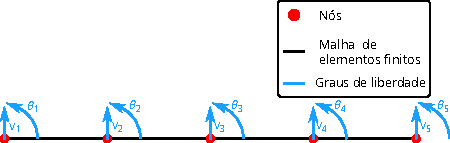
\includegraphics[scale=1.4]{Figures/6-Elemento_viga/Malha_Viga.pdf}
            \caption{Malha com elementos de vigas e seus graus de liberdade.}
            \label{fig:malha_viga}
        \end{figure}

        \begin{equation}
            v(\bar{x}) = \sum\limits_{i=1}^4 N_i(\bar{x}) a_i
        \end{equation}

        \begin{equation}
            \theta(\bar{x}) = \frac{dv}{dx} = \sum\limits_{i=1}^4 N_i'(\bar{x}) a_i
        \end{equation}

        Como há variáveis em $N_i(x)$ e em $N_i(x)$, para obtermos a mesma propriedade de que os coeficientes sejam correspondentes aos deslocamentos nodais, não utilizaremos os polinômios de Lagrange, mas uma outra família de polinômios, chamados \textbf{Polinômios de Hermite}.

        Os polinômios de Hermite são quatro polinômios de grau 3 com as seguintes propriedades:

        \begin{equation*}
            \begin{array}{cccc}
                N_1(\bar{x}_1) = 1, & N_1'(\bar{x}_1) = 0, & N_1(\bar{x}_2) = 0, & N_1'(\bar{x}_2) = 0\\
                N_2(\bar{x}_1) = 0, & N_2'(\bar{x}_1) = 1, & N_2(\bar{x}_2) = 0, & N_2'(\bar{x}_2) = 0\\
                N_3(\bar{x}_1) = 0, & N_3'(\bar{x}_1) = 0, & N_3(\bar{x}_2) = 1, & N_3'(\bar{x}_2) = 0\\
                N_4(\bar{x}_1) = 0, & N_4'(\bar{x}_1) = 0, & N_4(\bar{x}_2) = 0, & N_4'(\bar{x}_2) = 1
            \end{array}
        \end{equation*}

        De forma que tenhamos:

        \begin{equation*}
            \begin{array}{cccc}
                a_1 = v_1, & a_2 = \theta_1, & a_3 = v_2, & a_4 = \theta_2
            \end{array}
        \end{equation*}

        Os polinômios que resolvem este problema são:

        \begin{equation*}
            N_1(\bar{x}) = 2 \left(\frac{\bar{x}}{h_e}\right)^3 - 3 \left(\frac{\bar{x}}{h_e}\right)^2 + 1
        \end{equation*}

        \begin{equation*}
            N_2(\bar{x}) = h_e \left[ \left(\frac{\bar{x}}{h_e}\right)^3 - 2 \left(\frac{\bar{x}}{h_e}\right)^2 + \left(\frac{\bar{x}}{h_e}\right) \right]
        \end{equation*}

        \begin{equation*}
            N_3(\bar{x}) = -2 \left(\frac{\bar{x}}{h_e}\right)^3 + 3 \left(\frac{\bar{x}}{h_e}\right)^2
        \end{equation*}

        \begin{equation*}
            N_4(\bar{x}) = h_e \left[ \left(\frac{\bar{x}}{h_e}\right)^3 - \left(\frac{\bar{x}}{h_e}\right)^2 \right]
        \end{equation*}

        Suas derivadas são:

        \begin{equation*}
            N_1'(\bar{x}) = \frac{1}{h_e} \left[6 \left(\frac{\bar{x}}{h_e}\right)^2 - 6 \left(\frac{\bar{x}}{h_e}\right)\right] \rightarrow N_1''(\bar{x}) = \frac{1}{h_e^2} \left[12 \left(\frac{\bar{x}}{h_e}\right) - 6 \right]
        \end{equation*}

        \begin{equation*}
            N_2'(\bar{x}) = \left[ 3\left(\frac{\bar{x}}{h_e}\right)^2 - 4 \left(\frac{\bar{x}}{h_e}\right) + 1 \right]
            \rightarrow N_2''(\bar{x}) = \frac{1}{h_e} \left[6 \left(\frac{\bar{x}}{h_e}\right) -4 \right]
        \end{equation*}

        \begin{equation*}
            N_3'(\bar{x}) = \frac{1}{h_e} \left[-6 \left(\frac{\bar{x}}{h_e}\right)^2 + 6 \left(\frac{\bar{x}}{h_e}\right)\right] \rightarrow N_3''(\bar{x}) = \frac{1}{h_e^2} \left[-12 \left(\frac{\bar{x}}{h_e}\right) +6 \right]
        \end{equation*}

        \begin{equation*}
            N_4'(\bar{x}) = \left[ 3\left(\frac{\bar{x}}{h_e}\right)^2 - 2\left(\frac{\bar{x}}{h_e}\right) \right] \rightarrow N_4''(\bar{x}) = \frac{1}{h_e} \left[6 \left(\frac{\bar{x}}{h_e}\right) - 2 \right]
        \end{equation*}

        A Figura \ref{fig:hermite} mostra os polinômios de Hermite e suas derivadas avaliadas em um elemento com comprimento $h_e = 1$.

        \begin{figure}[h!]
            \begin{subfigure}{0.99\textwidth}
                \centering
                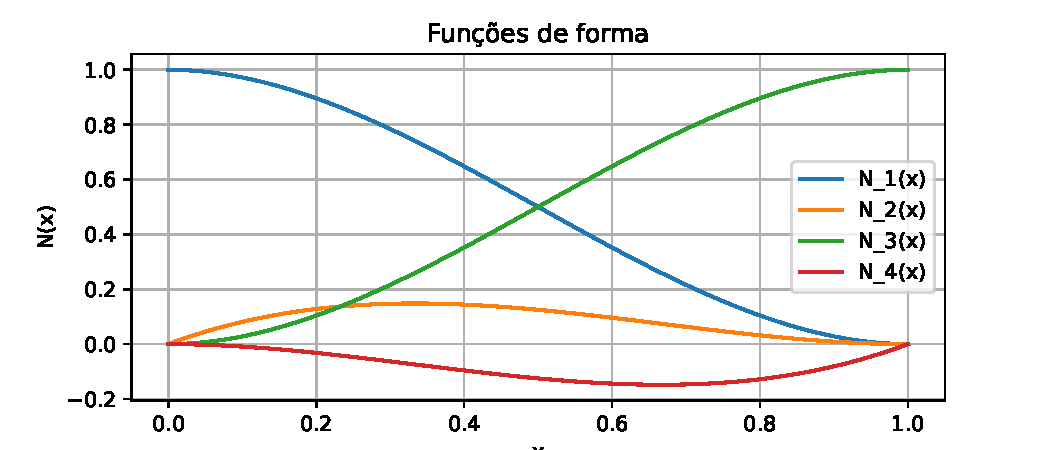
\includegraphics[scale=1]{Figures/6-Elemento_viga/Hermite.pdf}
                \caption{}
            \end{subfigure}
            \\
            \begin{subfigure}{0.99\textwidth}
                \centering
                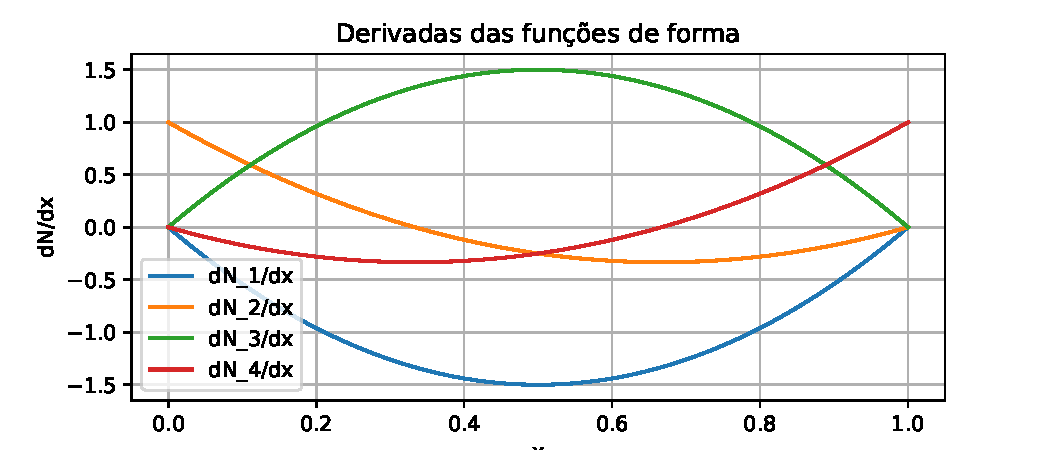
\includegraphics[scale=1]{Figures/6-Elemento_viga/Hermite_deriv.pdf}
                \caption{}
            \end{subfigure}
            \caption{Polinômios de Hermite usados na interpolação de elementos de viga. (a) polinômios de Hermite, (b) derivadas dos polinômios}
            \label{fig:hermite}
        \end{figure}

    \subsection{Resíduos ponderados e Galerkin}

        Com as funções de forma, podemos voltar à forma fraca. Na verdade, podemos definir uma solução aproximada com $v^h(x) \in V^h \subset V$, definida pelas funções de forma provenientes dos polinômios de Hermite. Com o método de Galerkin, as funções peso devem ser provenientes das mesmas funções de forma. Isto é:

        \begin{equation}
            v(\bar{x}) = N_1(\bar{x}) v_1 + N_2(\bar{x}) \theta_1 + N_3(\bar{x}) v_2 + N_4(\bar{x}) \theta_2 = 
            \begin{bmatrix}
                N_1 &
                N_2 &
                N_3 &
                N_4
            \end{bmatrix} 
            \begin{Bmatrix}
                v_1 \\
                \theta_1 \\
                v_2 \\
                \theta_2
            \end{Bmatrix}= 
            \mathbf{N} \mathbf{a}
        \end{equation}

        \begin{equation}
            \theta(\bar{x}) = N_1'(\bar{x}) v_1 + N_2'(\bar{x}) \theta_1 + N_3'(\bar{x}) v_2 + N_4'(\bar{x}) \theta_2 = 
            \frac{d\mathbf{N}}{dx} \mathbf{a}
        \end{equation}

        \begin{equation}
            w(\bar{x}) = N_1(\bar{x}) b_1 + N_2(\bar{x}) b_2 + N_3(\bar{x}) b_3 + N_4(\bar{x}) b_4 = 
            \mathbf{N} \mathbf{b}
        \end{equation}

        \begin{equation}
            \theta_w(\bar{x}) = N_1'(\bar{x}) b_1 + N_2'(\bar{x}) b_2 + N_3'(\bar{x}) b_3 + N_4'(\bar{x}) b_4 = 
            \frac{d\mathbf{N}}{dx} \mathbf{b}
        \end{equation}

        Substituindo essas expressões na forma fraca aproximada:

        
        \begin{equation*}
            \int_0^L \mathbf{b}^T \left(\frac{d^2\mathbf{N}^T}{dx^2} EI_{zz}\frac{d^2\mathbf{N}}{dx^2}\right)\mathbf{a} dx = 
        \end{equation*}

        \begin{equation}
            -\mathbf{b}^T \mathbf{N}(L)^T V_y(L) + \mathbf{b}^T \mathbf{N}(0)^T V_y(0) + \mathbf{b}^T \left.\frac{d\mathbf{N}^T}{dx}\right|_{x=L}M_z(L) - \mathbf{b}^T \left.\frac{d\mathbf{N}^T}{dx}\right|_{x=0}M_z(0)+ \int_0^L \mathbf{b}^T \mathbf{N}(x) q(x) dx
        \end{equation}

        Novamente, como a solução deve ser verificada para qualquer função $w(x)$, então ela deve valer para qualquer $b$. Portanto, devemos resolver o seguinte sistema linear:

        \begin{equation*}
            \left(\int_0^L \frac{d^2\mathbf{N}^T}{dx^2} EI_{zz}\frac{d^2\mathbf{N}}{dx^2} dx \right)\mathbf{a} = 
        \end{equation*}

        \begin{equation}
            -\mathbf{N}(L)^T V_y(L) + \mathbf{N}(0)^T V_y(0) + \left.\frac{d\mathbf{N}^T}{dx}\right|_{x=L}M_z(L) - \left.\frac{d\mathbf{N}^T}{dx}\right|_{x=0}M_z(0)+ \int_0^L \mathbf{N}(x) q(x) dx
        \end{equation}
        
    \subsection{Matriz elementar}

        Dado um elemento, a matriz de rigidez elementar será dada pelos quatro graus de liberdade do elemento:

        \begin{equation*}
            \mathbf{K}_e = \int_0^{h_e} \frac{d^2\mathbf{N}^T}{dx^2} EI_{zz}\frac{d^2\mathbf{N}}{dx^2} d\bar{x}
        \end{equation*}

        \begin{equation}
            \mathbf{K}_e = \int_0^{h_e} 
            \begin{Bmatrix}
                N_1'' \\
                N_2'' \\
                N_3'' \\
                N_4''
            \end{Bmatrix} 
             EI_{zz} 
             \begin{bmatrix}
                N_1'' &
                N_2'' &
                N_3'' &
                N_4''
            \end{bmatrix}  d\bar{x} =
            \int_0^{h_e}
            \mathbf{B}_e^T
            \mathbf{D}_e
            \mathbf{B}_e
            dx
        \end{equation}

        Se substituirmos os polinômios de Hermite e integrarmos, podemos obter matriz de rigidez deste elemento analiticamente:

        \begin{equation}
            \mathbf{K}_e = 
            \frac{EI_{zz}}{h_e^3}
            \begin{bmatrix}
                12   & 6h_e   & -12   & 6h_e   \\
                6h_e & 4h_e^2 & -6h_e & 2h_e^2 \\
                -12  & -6h_e  & 12    & -6h_e  \\
                6h_e & 2h_e^2 & -6h_e & 4h_e^2
            \end{bmatrix}
        \end{equation}


        Podemos fazer o mesmo para o vetor de forças. Integrando-a da seguinte forma:

        \begin{equation}
            \mathbf{f}_e = 
            \int_0^{h_e} 
            \begin{Bmatrix}
                N_1(\bar{x})\\
                N_2(\bar{x})\\
                N_3(\bar{x})\\
                N_4(\bar{x})
            \end{Bmatrix}
            q(x)
            dx
        \end{equation}

        Se considerarmos uma força distribuída uniforma $q_0$ vertical para cima:

        \begin{equation}
            \mathbf{f}_e = 
            \frac{q_0 h_e}{2}
            \begin{Bmatrix}
                1\\
                \frac{h_e}{6}\\
                1\\
                -\frac{h_e}{6}
            \end{Bmatrix}
        \end{equation}


    \subsection{Exemplo}

        Considere a viga da Figura \ref{fig:viga_exemplo_fem}. Assuma $EI_{zz} = 10^3 Nm^2$ e $L=10 m$.

        \begin{figure}[h!]
            \centering
            
\includegraphics[scale=1]{Figures/6-Elemento_viga/Exemplo.pdf}
            \caption{Viga a ser resolvida no exemplo de elementos finitos}
            \label{fig:viga_exemplo_fem}
        \end{figure}

        A solução analítica para essa viga é dada por:

        \begin{equation*}
            u_\text{an}(x) = \frac{1}{EI_{zz}} \left[-\frac{x^5}{120} + \frac{L^2}{12} x^3 - \frac{L^3}{6} x^2\right]
        \end{equation*}

        \begin{equation*}
            \theta_\text{an}(x) = \frac{1}{EI_{zz}} \left[-\frac{x^4}{24} + \frac{L^2}{4} x^2 - \frac{L^3}{3} x\right]
        \end{equation*}

        \begin{equation*}
            {V_y}_\text{an}(x) = -\frac{x^3}{6} + \frac{L^2}{2} x - \frac{L^3}{3}
        \end{equation*}

        \begin{equation*}
            {M_z}_\text{an}(x) = -\frac{x^2}{2} + \frac{L^2}{2}
        \end{equation*}

        Resolvendo por elementos finitos, com dois elementos, há seis graus de liberdade, dois para cada nó. O programa exemplo\_viga.py mostra resolve este problema por elementos finitos usando a biblioteca da disciplina. A Figura \ref{fig:exemplo_viga_mef} mostra o deslocamento, rotação, momento fletor e esforço cortante por elementos finitos e analíticos.

        \begin{figure}[h!]
            \begin{subfigure}{0.46\textwidth}
                \centering
                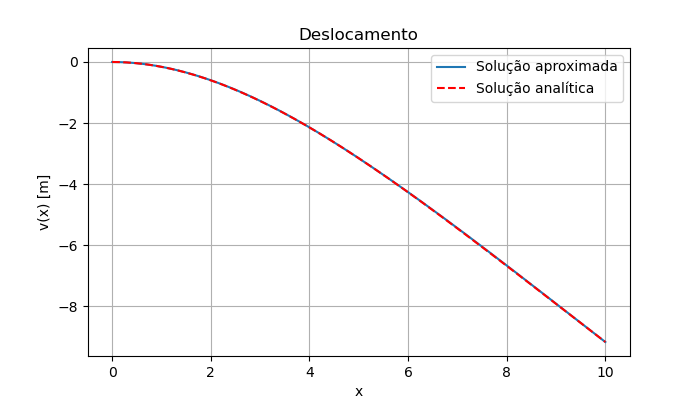
\includegraphics[scale=0.5]{Figures/6-Elemento_viga/deslocamento.png}
                \caption{}
            \end{subfigure}
            ~
            \begin{subfigure}{0.46\textwidth}
                \centering
                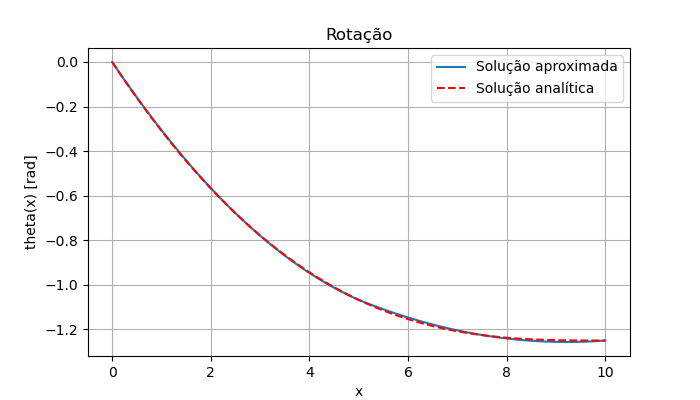
\includegraphics[scale=0.5]{Figures/6-Elemento_viga/rotacao.png}
                \caption{}
            \end{subfigure}\\
            \begin{subfigure}{0.46\textwidth}
                \centering
                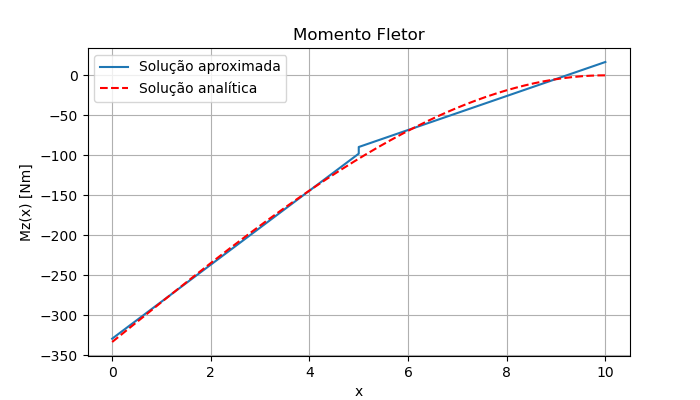
\includegraphics[scale=0.5]{Figures/6-Elemento_viga/fletor.png}
                \caption{}
            \end{subfigure}
            ~
            \begin{subfigure}{0.46\textwidth}
                \centering
                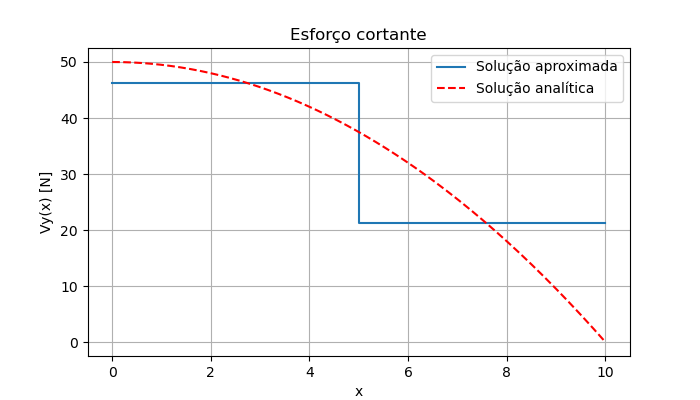
\includegraphics[scale=0.5]{Figures/6-Elemento_viga/cortante.png}
                \caption{}
            \end{subfigure}\\
            \caption{Solução por elementos finitos e analítica do problema de barra. (a) deslocamento, (b) rotação, (c) momento fletor, (d) esforço cortante.}
            \label{fig:exemplo_viga_mef}
        \end{figure}

    \subsection{Elemento de pórtico}

        O elemento de viga e o elemento de barra descrevem o comportamento de um elemento em duas direções diferentes. A barra descreve a tração e a compressão do elemento, e a viga descreve sua flexão. Como ambos os modelos são lineares, podemos considerar um elemento que combine os dois comportamentos pelo princípio da superposição.

        Um elemento de barra possui apenas um grau de liberdade em cada nó (deslocamento $x$), enquanto que o de viga tem dois graus de liberdade (deslocamento $y$ e rotação $\theta_z$). Podemos definir um elemento de pórtico com três graus de liberdade por nó (Figura \ref{fig:portico}).

        \begin{figure}[h!]
            \centering
            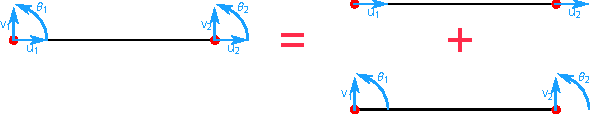
\includegraphics[scale=1.4]{Figures/6-Elemento_viga/Portico.pdf}
            \caption{Elemento de pórtico pela superposição de barra e viga}
            \label{fig:portico}
        \end{figure}

        Por ser um elemento que combina o comportamento dos outros dois, de forma desacoplada, isto é, a barra não modifica o comportamento da viga e vice-versa, podemos apenas concatenar as matrizes de rigidez e os vetores de força:

        \begin{equation}
            \mathbf{K_e}=
            \frac{EA}{h_e}
            \begin{bmatrix}
                1 & 0 & 0 & -1 & 0 & 0\\
                0 & 0 & 0 & 0 & 0 & 0\\
                0 & 0 & 0 & 0 & 0 & 0\\
                -1 & 0 & 0 & 1 & 0 & 0\\
                0 & 0 & 0 & 0 & 0 & 0\\
                0 & 0 & 0 & 0 & 0 & 0\\
            \end{bmatrix}+
            \frac{EI_{zz}}{h_e^3}
            \begin{bmatrix}
                0 & 0 & 0 & 0 & 0 & 0\\
                0 & 12   & 6h_e   & 0 &  -12   & 6h_e   \\
                0 & 6h_e & 4h_e^2 & 0 &  -6h_e & 2h_e^2 \\
                0 & 0 & 0 & 0 & 0 & 0\\
                0 & -12  & -6h_e  & 0 &  12    & -6h_e  \\
                0 & 6h_e & 2h_e^2 & 0 &  -6h_e & 4h_e^2
            \end{bmatrix}
        \end{equation}

        \begin{equation}
            \mathbf{K_e}=
            \begin{bmatrix}
                k_b & 0 & 0 & -k_b & 0 & 0\\
                0 & 12 k_v   & 6h_e k_v   & 0 &  -12k_v   & 6h_e k_v   \\
                0 & 6h_e k_v & 4h_e^2k_v & 0 &  -6h_e k_v & 2h_e^2k_v \\
                -k_b & 0 & 0 & k_b & 0 & 0\\
                0 & -12k_v  & -6h_e k_v  & 0 &  12k_v    & -6h_ek_v \\
                0 & 6h_e k_v & 2h_e^2k_v & 0 &  -6h_e k_v & 4h_e^2k_v 
            \end{bmatrix}
        \end{equation}

        \noindent no qual $k_b = \frac{EA}{h_e}$ e $k_v = \frac{EI_{zz}}{h_e^3}$.

        O sistema, portanto, fica:

        \begin{equation}
            \begin{bmatrix}
                k_b & 0 & 0 & -k_b & 0 & 0\\
                0 & 12 k_v   & 6h_e k_v   & 0 &  -12k_v   & 6h_e k_v   \\
                0 & 6h_e k_v & 4h_e^2k_v & 0 &  -6h_e k_v & 2h_e^2k_v \\
                -k_b & 0 & 0 & k_b & 0 & 0\\
                0 & -12k_v  & -6h_e k_v  & 0 &  12k_v    & -6h_e k_v \\
                0 & 6h_e k_v & 2h_e^2k_v & 0 &  -6h_e k_v & 4h_e^2k_v 
            \end{bmatrix}
            \begin{Bmatrix}
                u_1\\
                v_1\\
                \theta_1\\
                u_2\\
                v_2\\
                \theta_2
            \end{Bmatrix}
            =
            \begin{Bmatrix}
                f_{x_1}\\
                f_{y_1}\\
                m_1\\
                f_{x_2}\\
                f_{y_2}\\
                m_2
            \end{Bmatrix}
        \end{equation}

        O elemento de pórtico, no entanto, nem sempre estará alinhado ao sistema de coordenadas globais. Portanto, considere o elemento da Figura \ref{fig:portico_rotacionado}, que em coordenadas locais está alinhado ao sistema de coordenadas $\bar{x}\bar{y}$. Desejamos obter a matriz de rigidez deste sistema em coordenadas globais $xy$.

        \begin{figure}[h]
            \centering
            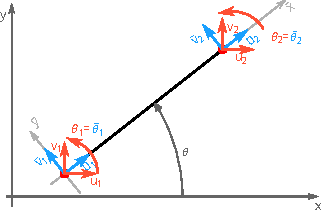
\includegraphics[scale=1.8]{Figures/6-Elemento_viga/Rotacionado.pdf}
            \caption{Elemento de pórtico rotacionado por um ângulo $\theta$}
            \label{fig:portico_rotacionado}
        \end{figure}

        Um vetor no sistema local pode ser transformado ao sistema global multiplicando-o por uma matriz de rotação $\mathbf{R}$:

        \begin{equation}
            \mathbf{\bar{u}} = 
            \begin{Bmatrix}
                \bar{u}\\
                \bar{v}\\
                \bar{\theta}
            \end{Bmatrix}
            =
            \begin{bmatrix}
                \text{cos} \theta & \text{sen} \theta & 0\\
                -\text{sen} \theta & \text{cos} \theta & 0\\
                0 & 0 & 1
            \end{bmatrix}
            \begin{Bmatrix}
                u\\
                v\\
                \theta
            \end{Bmatrix}=
            \mathbf{R} \mathbf{u}
        \end{equation}

        Matrizes de rotação são chamadas \textbf{matrizes ortogonais}. Uma propriedade de matrizes ortogonais é que a sua inversa é igual a sua transposta. O leitor interessado pode verificar essa propriedade na matriz acima ou na matriz de rotação 3D. Portanto, a transformação inversa é dada por:

        \begin{equation}
            \mathbf{u} = \mathbf{R}^T \mathbf{\bar{u}}
        \end{equation}

        Para um dado elemento, podemos escrever a matriz de rotação:

        \begin{equation}
            \mathbf{\bar{u}} = 
            \begin{Bmatrix}
                \bar{u}_1\\
                \bar{v}_1\\
                \bar{\theta}_1\\
                \bar{u}_2\\
                \bar{v}_2\\
                \bar{\theta}_2
            \end{Bmatrix}
            =
            \begin{bmatrix}
                \text{cos} \theta & \text{sen} \theta & 0 & 0 & 0 & 0\\
                -\text{sen} \theta & \text{cos} \theta & 0 & 0 & 0 & 0\\
                0 & 0 & 1 & 0 & 0 & 0\\
                0 & 0 & 0 & \text{cos} \theta & \text{sen} \theta & 0\\
                0 & 0 & 0 & -\text{sen} \theta & \text{cos} \theta & 0\\
                0 & 0 & 0 & 0 & 0 & 1
            \end{bmatrix}
            \begin{Bmatrix}
                u_1\\
                v_1\\
                \theta_1\\
                u_2\\
                v_2\\
                \theta_2\\
            \end{Bmatrix}=
            \mathbf{R}_e \mathbf{u}
        \end{equation}

        O sistema em coordenadas locais pode ser convertido para o sistema em coordenadas globais da seguinte forma:

        \begin{equation*}
            \mathbf{\bar{K}}_e \mathbf{\bar{u}} = \mathbf{\bar{f}}_e
        \end{equation*}

        Pre-multiplicando por $\mathbf{R}^T$ e substituindo a expressão de $mathbf{\bar{u}}$:

        \begin{equation*}
            \mathbf{R}_e^T \mathbf{\bar{K}}_e \mathbf{R}_e \mathbf{u}_e = \mathbf{R}_e^T \mathbf{\bar{f}}_e
        \end{equation*}
        
        \begin{equation*}
            \mathbf{K}_e \mathbf{u}_e = \mathbf{f}_e
        \end{equation*}

        \noindent no qual a matriz então pode ser encontrada como:

        \begin{equation*}
            \mathbf{K}_e = \mathbf{R}_e^T \mathbf{\bar{K}}_e \mathbf{R}_e
        \end{equation*}

        Com relação ao vetor de força, as forças normalmente já são descritas em função do sistema de coordenadas globais, então não é necessária a transformação, neste caso. Entretanto, se a força estiver rotacionada com o elemento, podemos transformá-la de forma similar.

        Finalmente, para o elemento definido pelos pontos $(x_1,y_1)$ e $(x_2,y_2)$, lembre-se que podemos encontrar seu comprimento e ângulo como:

        \begin{equation*}
            h_e = \sqrt{\left(x_2-x_1\right)^2+\left(y_2-y_1\right)^2}
        \end{equation*}

        \begin{equation*}
            \theta_e = \text{tan}^{-1}\left(\frac{y_2-y_1}{x_2-x_1}\right)
        \end{equation*}

        Para o ângulo, devemos nos atentar na programação. Como a função tangente é periódica em $\pi$, usar uma função do tipo \textit{atan()} não é suficiente para obtermos em qual quadrante o ângulo realmente está. Portanto, devemos usar funções do tipo \textit{atan2()}, que também verifica os sinais do denominador e numerador para identificar em qual quadrante o ângulo está.


        Com este elemento de pórtico, podemos resolver sistemas com vários elementos conectados entre si. Por exemplo, se removermos o termo de viga (colocar $k_v=0$ e tirar os graus de liberdade $\theta_z$), podemos montar e resolver um sistema de treliças.

        Portanto, para cada elemento, aplicamos a rotação dele na matriz de rigidez, e montamos no sistema global seguindo o procedimento de montagem mostrado anteriormente.

    \subsection{Exemplo de sistema de pórticos - treliça}

        Considere a treliça da Figura \ref{fig:trelica_ex}. Encontre os deslocamentos dos nós e as tensões em cada barra. Considere que cada barra tem $A = 10^{-5} m$.

        \begin{figure}[h!]
            \centering
            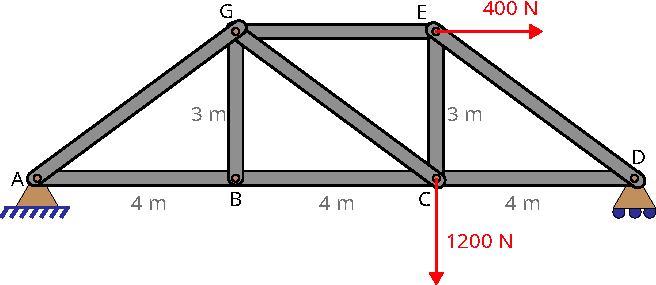
\includegraphics[scale=1]{Figures/6-Elemento_viga/Trelica_exemplo.pdf}
            \caption{Exemplo de problema de treliça}
            \label{fig:trelica_ex}
        \end{figure}

        \subsubsection*{Solução}

        Resolvendo analiticamente, usando equações de equilíbrio da Estática, obtemos as forças de cada barra, e, consequentemente, suas tensões:

        \begin{table}[h!]
            \centering
            \caption{Forças e tensões analíticas do problema de treliça}
            \begin{tabular}{|c|c|c|}
            \hline
            \rowcolor[HTML]{9B9B9B} 
            Barra & Força {[}N{]} & Tensão {[}MPa{]} \\ \hline
            \rowcolor[HTML]{EFEFEF} 
            AB    & 800           & 80               \\ \hline
            \rowcolor[HTML]{FFFFFF} 
            BC    & 800           & 80               \\ \hline
            \rowcolor[HTML]{EFEFEF} 
            CD    & 1200          & 120              \\ \hline
            \rowcolor[HTML]{FFFFFF} 
            DE    & -1500         & -150             \\ \hline
            \rowcolor[HTML]{EFEFEF} 
            EG    & -800          & -80              \\ \hline
            \rowcolor[HTML]{FFFFFF} 
            AG    & -500          & -50              \\ \hline
            \rowcolor[HTML]{EFEFEF} 
            BG    & 0             & 0                \\ \hline
            \rowcolor[HTML]{FFFFFF} 
            CG    & 500           & 50               \\ \hline
            \rowcolor[HTML]{EFEFEF} 
            CE    & 900           & 90               \\ \hline
            \end{tabular}
        \end{table}

        Para resolver por elementos finitos, foi utilizado o programa exemplo\_trelica.py. O deslocamento nodal de cada grau de liberdade, usando a numeração seguindo os nós em ordem alfabética. O mapa de tensões encontrado é mostrado na Figura \ref{fig:ex_trelica_tensao}.

        \begin{figure}[h!]
            \centering
            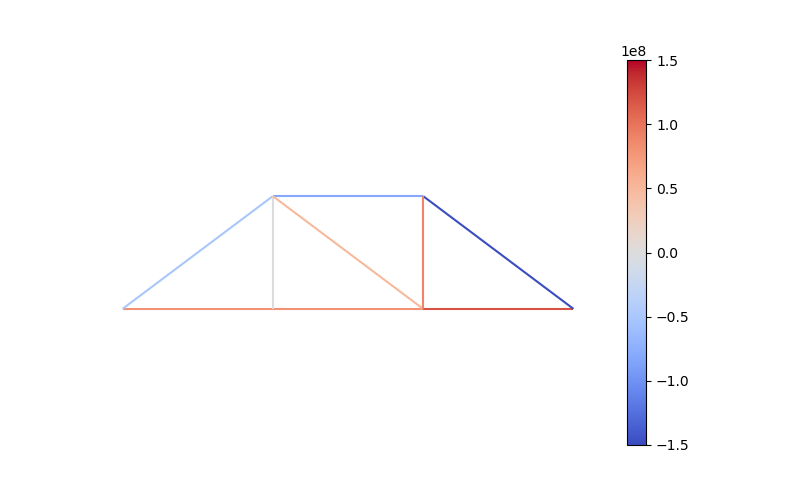
\includegraphics[scale=0.8]{Figures/6-Elemento_viga/tensao_trelica.png}
            \caption{Tensões nas barras. Tensão em Pa.}
            \label{fig:ex_trelica_tensao}
        \end{figure}




    
